\documentclass[crop,class=article]{standalone}
%----------------------------Preamble-------------------------------%
\usepackage{tikz}                   % Drawing/graphing tools.
\usetikzlibrary{
    angles,                 % Drawing angles within triangles.
    arrows.meta,            % Latex and Stealth arrows.
    quotes                  % Adding labels to angles.
}
%--------------------------Main Document----------------------------%
\begin{document}
    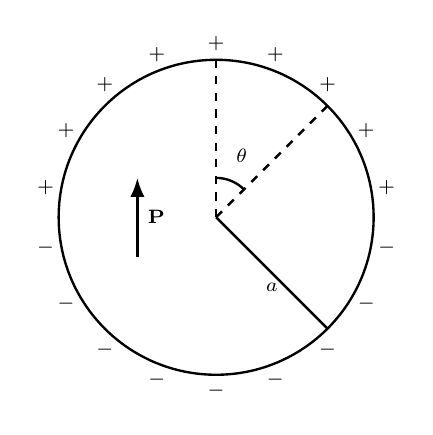
\begin{tikzpicture}[font=\scriptsize,>=Latex,line width=0.3mm]
        \draw (0,0) circle (2);
        \node (O) at (0,0) {};
        \node (A) at (0,2) {};
        \node (B) at (1.414,1.414) {};
        \draw[dashed] (0,0) to (0,2);
        \draw[dashed] (0,0) to (1.414,1.414);
        \draw (0,0) to node[below] {$a$} (1.414,-1.414);
        \pic[%
            draw=black,
            "\scriptsize{${\theta}$}",
            angle eccentricity=1.7,
            angle radius =0.5cm
        ]   {angle = B--O--A};
        \draw[->] (-1,-0.5) to node[right] {$\mathbf{P}$} (-1,0.5);
        \foreach \a in {1,3,...,17}{
            \draw (\a*360/36: 2.2) node{$+$};
            \draw (\a*360/36+180: 2.2) node{$-$};
        }
    \end{tikzpicture}
\end{document}